\documentclass[12pt,openany,oneside,a4paper]{abntex2}
\usepackage[portuguese]{babel}
\usepackage{amsmath}
\usepackage{amssymb}
\usepackage{graphicx}
\usepackage{lipsum}
\usepackage{circuitikz}
\usepackage{icomma}
\usepackage{tikz}
\usepackage{float}
\usepackage{circuitikz}
\documentclass{book} % ou report, article etc.
\usepackage[utf8]{inputenc}
\usepackage{titlesec}
\usepackage{caption}
\usepackage{float}

% Redefine o formato das seções para usar letras
\renewcommand{\thesection}{\alph{section})}

\titulo{Atividades Teóricas da C1}
\autor{Matheus Amaral da Costa}
\data{Junho de 2025}
\instituicao{
  Centro Universitário FAESA
  \par
  Engenharia da Computação}
\local{Vitória, ES}

\begin{document}

\imprimircapa
\imprimirfolhaderosto*

\tableofcontents

\chapter{Questão 1}
\section{}
\subsection{Considerações Iniciais}
Considerar que os capacitores estão "abertos".

\subsection{Representação do Circuito}
\begin{center}
    \begin{circuitikz}[american]
        \draw (3,2) node[npn, anchor=B, scale=1.5](Q1){};
        \draw (0,0) to node[ground]{} (0,0) to[sV, a=$v_{in}$,v=$1mV$] (0,2)
          to[C] (Q1.B);
        \draw (Q1.B) to[R, , a=$R_1$,l=$10k\Omega$]
              ++(0,3) -- ++(0.5,0) -- ++(0,0.5)
              node[ocirc](Vcc){$+10_{Vcc}$} 
              (Vcc) ++(0,-0.5) -- ++(0.75,0) to[R, a=$R_C$, l=$3{,}6k\Omega$] (Q1.C);
        \draw (Q1.C) to[C] (8,3.2) to[R, a=$R_L$,l=$10k\Omega$] (8,0)
              node[ground]{};
        \draw (Q1.B) to[R, l=$R_2$, a=$2{,}2k\Omega$] (3,0)
              node[ground]{};
        \draw (Q1.E) -- (4.3, 0) to[R, a=$R_E$, l=$1k\Omega$] (4.3,-2) node[ground]{};
        \draw (Q1.E) to[C] (6.3,0.88);
        \draw (6.3,0.88) -- (6.3,-1) node[ground]{};
        \node at (4,-3) {\large \textbf{Figura 1 - Circuito Elétrico}};
    \end{circuitikz}
\end{center}

\subsection{Dados do Circuito}
\begin{itemize}
    \item $V_{CC} = 10V$
    \item $R_1 = 10\,\text{k}\Omega$
    \item $R_2 = 2{,}2\,\text{k}\Omega$
    \item $R_C = 3{,}6 \, \text{k}\Omega$
    \item $R_E = 1 \, \text{k}\Omega$
    \item $R_L = 10 \, \text{k}\Omega$
\end{itemize}

\subsection{Determinação de $V_B$}
\[
V_B = V_{CC} \times \left(\frac{R_2}{R_1 + R_2}\right)
\]
\[
V_B = 10 \times (\frac{2{,}2 \times 10^3}{12{,}2 \times 10^3})
\]
\[
\tikz[baseline]{\node[draw=red, thick, rounded corners] {$V_B = 1{,}8\,V$};}
\]

\subsection{Cálculo de $I_E$}
Aplicando LKT na malha $\alpha$, tem-se:
\[
V_B - V_{BE} - R_E \cdot I_E = 0
\]
Se o diodo é de Silício, tem-se que $V_{BE} = 0{,}7V$, logo:
\[
1{,}8 - 0{,}7 - 1000 \cdot I = 0 \implies I_E = \frac{1{,}1}{1000} \implies \tikz[baseline]{\node[draw=red, thick, rounded corners] {$I_E = 1{,}1 \, \text{mA}$};}
\]

\subsection{Cálculo de $I_C$}
Para $\beta >= 100$, temos que $I_C \approx I_E \implies \tikz[baseline]{\node[draw=red, thick, rounded corners] {$I_C = 1{,}1 \, \text{mA}$};}$

\subsection{Cálculo de $I_B$}
Adotando $\beta$ = 100, temos: 
\[
I_B = \frac{I_C}{\beta} = \frac{1{,}1 \times 10^3}{100} \implies \tikz[baseline]{\node[draw=red, thick, rounded corners] {$I_B = 11 \, \text{µA}$};}
\]

\subsection{Cálculo do $I_C$ de Saturação}
\[
I_{Cmáx} = \frac{V_{CC}}{R_C + R_E} = \frac{10}{4{,}6 \times 10^3} \implies \tikz[baseline]{\node[draw=red, thick, rounded corners] {$I_{Cmáx} = 2{,}17 \, \text{mA}$};}
\]

\subsection{Cálculo de $V_{C}$}
Sabe-se que:
\[
V_{C} = V_{CC} - R_{C} I_{C} \implies V_{C} = 10 - 3,6k \cdot 1,1m \therefore \tikz[baseline]{\node[draw=red, thick, rounded corners] {$V_{C} = 6{,}04\,\text{V}$};}
\]

\subsection{Cálculo de $V_{BB}$}
\[
V_{BB} = \frac{R_{2}}{R_{1} + R_{2}} \cdot V_{CC}
\implies
V_{BB} = \frac{2,2k}{10k + 2,2k} \cdot 10
\implies
\tikz[baseline]{\node[draw=red, thick, rounded corners] {$V_{BB} = 1,8\,\text{V}$};}
\]

\subsection{Cálculo de $V_{E}$}
Sabe-se que:
\[
V_{E} = V_{BB} - V_{BE} \implies V_{E} = 1,8 - 0,7 \therefore \tikz[baseline]{\node[draw=red, thick, rounded corners] {$V_{E} = 1{,}1\,\text{V}$};}
\]

\subsection{Cálculo do $V_{CE}$}
\[
V_{CE} = V_{CC} - R_C I_C - R_E I_E
\]
\[
V_{CE} = 10 - (R_C + R_E) \cdot 1{,}1 \times 10^{-3} \implies V_{CE} = 10 - 5{,}06 \implies \tikz[baseline]{\node[draw=red, thick, rounded corners] {$V_{CE} = 4{,}94 \, \text{V}$};}
\]

\subsection{Gráfico $I_{C}$ x $V_{CE}$}
\begin{center}
    \begin{tikzpicture}
        \draw[->] (0,0) -- (5,0) node[right] {$V_{CE}$};
        \draw[->] (0,0) -- (0,5) node[above] {$I_C$};
        \draw[thick] (4,0) -- (0,4) node[left] {Saturação};
        \node at (4,-0.3) {Corte};
        \node at (3,2.3) {Operação};
        \node at (2.5,-1) {\large \textbf{Figura 2 - Gráfico $I_C$ x $V_{CE}$}};
    \end{tikzpicture}
\end{center}

\subsection{Conclusão}
Devido ao fato de $I_{C}$ ser menor que 2{,}17 mA ($I_{C\text{máx}}$) e ser diferente de zero, a configuração está funcionando como um amplificador.

\section{}
Adotando $\pi = 3,14$ e não atribuindo valor à frequência (forma literal)

\subsection{Cálculo do $R_{1} || R_{2}$}
\[
R_{1} || R_{2} = \frac{R_{1} \cdot R_{2}}{R_{1} + R_{2}} \implies R_{1} || R_{2} = \frac{10k \cdot 2,2k}{10k + 2,2k} \therefore \tikz[baseline]{\node[draw=red, thick, rounded corners] {$R_{1} || R_{2} \approx 1803{,}28\,\Omega$};}
\]

\subsection{Cálculo do $C_{1}$}
\[
C_{1} \geq \frac{1}{2\pi0,1(R_{1} || R_{2})f} \implies C_{1} \geq \frac{1}{2\pi0,1(1803,28)f} \therefore \tikz[baseline]{\node[draw=red, thick, rounded corners] {$C_{1} \geq (8{,}71f)\,\text{mF}$};}
\]

\subsection{Cálculo do $C_{2}$ (\textit{bypass})}
\[
C_{2} \geq \frac{1}{2\pi0,1R_{E}f} \implies C_{2} \geq \frac{1}{2\pi0,1(1000)f} \therefore \tikz[baseline]{\node[draw=red, thick, rounded corners] {$C_{2} \geq (1{,}59f)\,\text{mF}$};}
\]

\subsection{Cálculo do $R_{C} || R_{L}$}
\[
R_{C} || R_{L} = \frac{R_{C} \cdot R_{L}}{R_{C} + R_{L}} \implies R_{C} || R_{L} = \frac{3,6k \cdot 10k}{3,6k + 10k} \therefore \tikz[baseline]{\node[draw=red, thick, rounded corners] {$R_{C} || R_{L} \approx 2647{,}06\,\Omega$};}
\]

\subsection{Cálculo do $C_{3}$}
\[
C_{3} \geq \frac{1}{2\pi0,1(R_{C} || R_{L})f} \implies C_{3} \geq \frac{1}{2\pi0,1(2647,06)f} \therefore \tikz[baseline]{\node[draw=red, thick, rounded corners] {$C_{3} \geq (6{,}02f)\cdot 10^{-4}\,\text{F}$};}
\]

\section{}

\subsection{Cálculo de $re'$}
\[
re' = \frac{25mV}{I_{E}} \implies re' = \frac{25mV}{1,1mA} \therefore \tikz[baseline]{\node[draw=red, thick, rounded corners] {$re' \approx 22{,}72\,\Omega$};}
\]

\subsection{Cálculo da impedância de entrada da base ($Z_{in_{\text{B}}}$)}
\[
Z_{in_{\text{B}}} = \beta \cdot re' \implies Z_{in_{\text{B}}} = 100 \cdot 22,72 \therefore \tikz[baseline]{\node[draw=red, thick, rounded corners] {$Z_{in_{\text{B}}} = 2{,}272\,k\Omega$};}
\]

\subsection{Cálculo do $R_{B}$}
\[
R_{B} = R_{1} || R_{2} \implies R_{B} = \frac{R_{1} \cdot R_{2}}{R_{1} + R_{2}} \implies R_{B} = \frac{10k \cdot 2,2k}{10k + 2,2k} \therefore \tikz[baseline]{\node[draw=red, thick, rounded corners] {$R_{B} \approx 1803{,}28\,\Omega$};}
\]

\subsection{Cálculo da impedância de entrada ($Z_{in}$)}
\[
Z_{in} = R_{B} || Z_{in_{\text{B}}} \implies Z_{in} = \frac{1,80328k \cdot 2,272k}{1,80328k + 2,272k} \therefore \tikz[baseline]{\node[draw=red, thick, rounded corners] {$Z_{in} \approx 1\,k\Omega$};}
\]

\subsection{Cálculo da impedância de saída}
\[
Z_{out} \approx R_{C} \therefore \tikz[baseline]{\node[draw=red, thick, rounded corners] {$Z_{out} = 3{,}6\,k\Omega$};}
\]Sim, temos um amplificador de pequenos sinais devido, não só a análise das impedâncias de entrada e saída, mas também pelo fato de $V_{g} = 1\,mV$, valor esse tido como pequeno.

\section{}

\subsection{Cálculo de $r_{c}$}
\[
r_{c} = R_{c} || R_{L} \implies r_{c} = \frac{3,6k \cdot 10k}{3,6k + 10k} \therefore \tikz[baseline]{\node[draw=red, thick, rounded corners] {$r_{c} \approx 2647{,}06\,\Omega$};}
\]

\subsection{Cálculo de $re'$}
\[
re' = \frac{25mV}{I_{E}} \implies re' = \frac{25mV}{1,1mA} \therefore \tikz[baseline]{\node[draw=red, thick, rounded corners] {$re' \approx 22{,}72\,\Omega$};}
\]

\subsection{Cálculo do ganho de sinal}
\[
A_{v} = \frac{r_{c}}{re'} \implies A_{v} = \frac{2647,06}{22,72} \therefore \tikz[baseline]{\node[draw=red, thick, rounded corners] {$A_{v} \approx 116{,}51$};}
\]

\section{}
\subsection{Esboço}
\begin{center}
\begin{tikzpicture}[scale=1.2]
    % Eixos
    \draw[->] (-1.5,0) -- (5.5,0) node[right] {$t\,\text{(s)}$};
    \draw[->] (0,-1.5) -- (0,1.8) node[above] {$V(V)$};

    % Parte tracejada à esquerda
    \draw[dashed, domain=-1.5:0, samples=100, smooth] 
        plot(\x, {sin(2*pi*\x r)});

    % Parte principal (contínua)
    \draw[thick, domain=0:4.5, samples=200, smooth] 
        plot(\x, {sin(2*pi*\x r)});

    % Parte tracejada à direita
    \draw[dashed, domain=4.5:5.2, samples=100, smooth] 
        plot(\x, {sin(2*pi*\x r)});
\end{tikzpicture}
\\
\large \textbf{Figura 3 - Gráfico $V$ x $t$}
\end{center}

\subsection{Simulação no MULTISIM}
\begin{figure}[H]
    \centering
    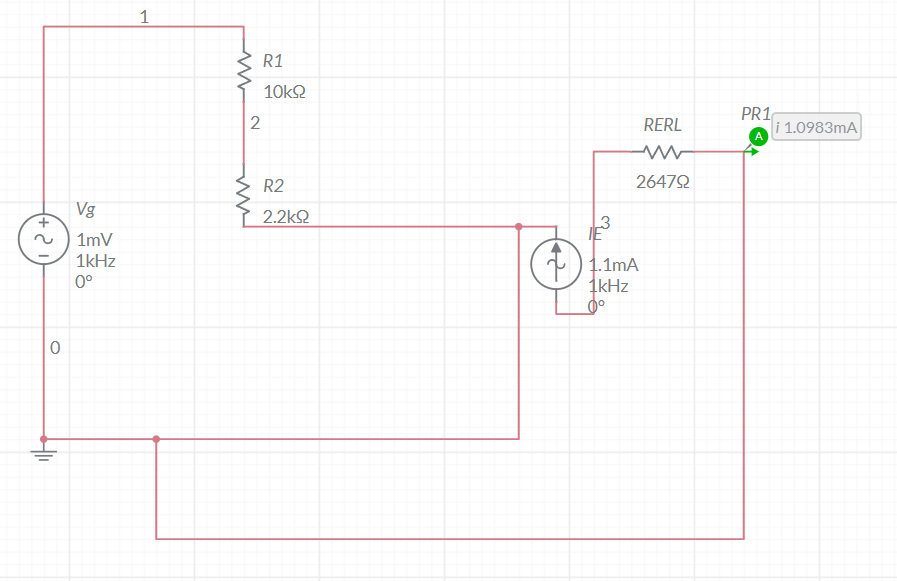
\includegraphics[width=1\textwidth]{Simulacao11.png}
    \large \textbf{Figura 4 - Simulação da Questão 1}
\end{figure}

\begin{figure}[H]
    \centering
    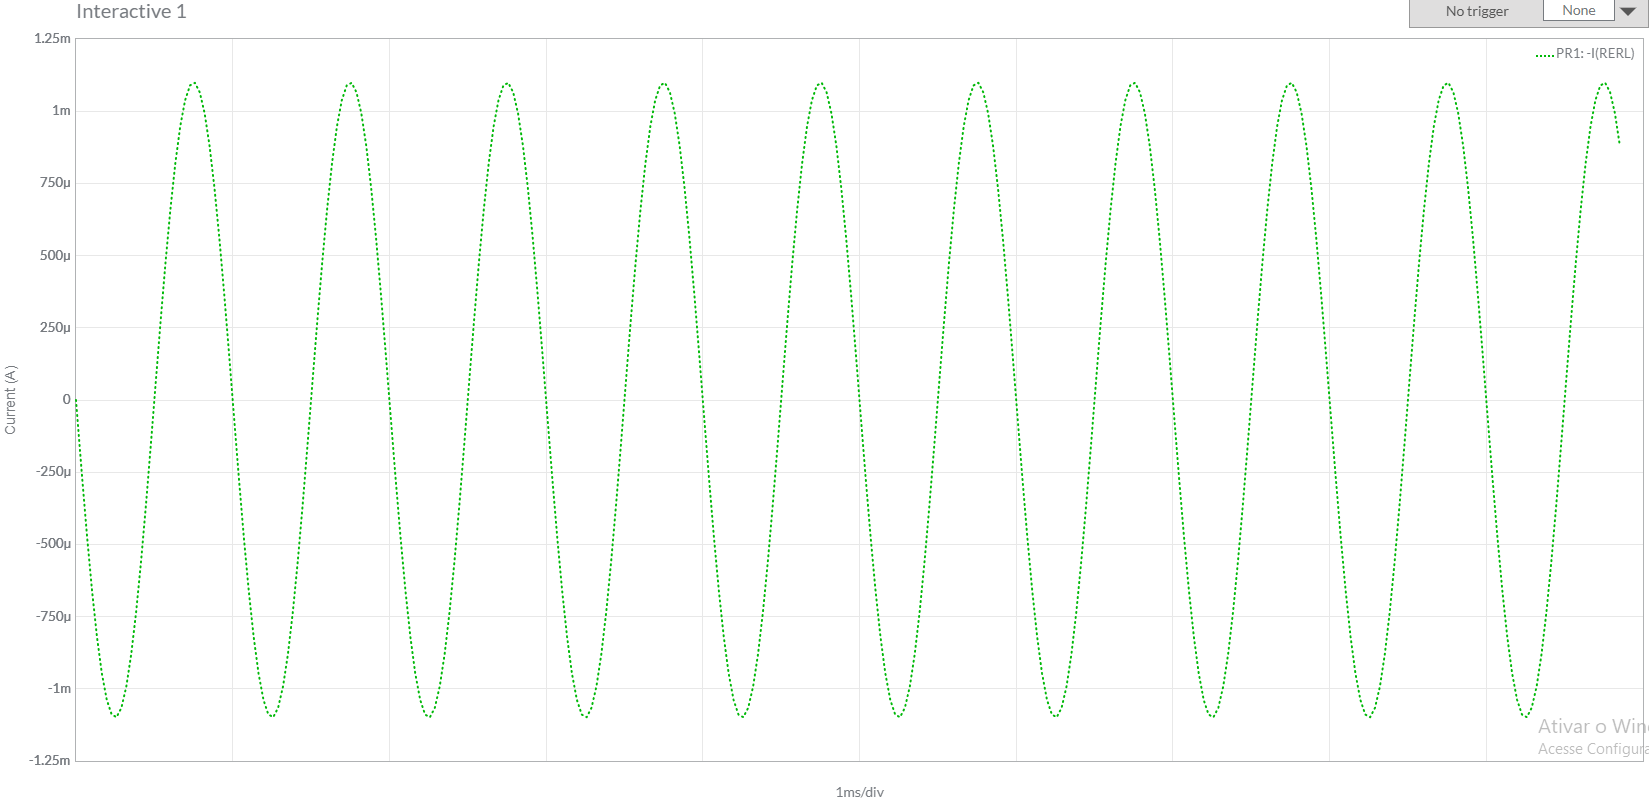
\includegraphics[width=1\textwidth]{Simulacao12.png}
    \large \textbf{Figura 5 - Simulação da Questão 1}
\end{figure}


\chapter{Questão 2}
\section{}

\subsection{Simplificação da Polarização por Divisor de Tensão}
\begin{center}
    \begin{tikzpicture}
    	% Paths, nodes and wires:
    	\draw node[ground] at (3, 6) {};
    	\draw node[ground] at (4.5, 6) {};
    	\draw node[ground] at (6, 6) {};
    	\draw (3, 6) to[american resistor, l={$R2$}, label distance=0.02cm] (3, 7.875);
    	\draw (4.5, 6) to[american resistor, l={$RE$}, label distance=0.02cm] (4.5, 7.5);
    	\draw node[npn] at (4.5, 9) {};
    	\draw (3, 7.875) -| (3, 9) -- (3.66, 9);
    	\draw (4.5, 8.23) -| (4.5, 7.5);
    	\draw (3, 9.77) to[american resistor, l={$R1$}, label distance=0.02cm] (3, 11.52);
    	\draw (4.5, 9.77) to[american resistor, l={$RC$}, label distance=0.02cm] (4.5, 11.52);
    	\draw (3, 11.52) -- (4.5, 11.52);
    	\draw (3, 9.77) -| (3, 9);
    	\draw (6, 9.375) to[battery, l={$VCC$}, label distance=0.02cm] (6, 8.625);
    	\draw (6, 6) -| (6, 8.625);
    	\draw (4.5, 11.52) -| (6, 11.5) -| (6, 9.375);
    	\draw node[circ] (N1) at (3, 9) {} node[anchor=south east] at (N1.north west){$VBB$};
    \end{tikzpicture}
    \\
    \textbf{Figura 6 - Circuito Elétrico Simplificado}
\end{center}

\subsection{Dados do Circuito}
\begin{itemize}
    \item $V_{CC} = 10\,V$ 
    \item $R_{1} = 10\,{k}\Omega$ 
    \item $R_{2} = 2,2\,{k}\Omega$
    \item $R_{C} = 3,6\,{k}\Omega$
    \item $R_{E} = 1\,{k}\Omega$
    \item $R_{L} = 10\,{k}\Omega$
    \item $R_{G} = 600 \ \Omega$
    \item $\beta = 100$
\end{itemize}
    
\subsection{Cálculo de $V_{BB}$}
\[
V_{BB} = \frac{R_{2}}{R_{1} + R_{2}} \cdot V_{CC}
\implies
V_{BB} = \frac{2,2k}{10k + 2,2k} \cdot 10
\implies
\tikz[baseline]{\node[draw=red, thick, rounded corners] {$V_{BB} = 1,8\,\text{V}$};}
\]

\subsection{Cálculo de $I$}
\[
I = \frac{V_{CC}}{R_{1} + R_{2}} \implies
I = \frac{10}{10k + 2,2k} \implies
\tikz[baseline]{\node[draw=red, thick, rounded corners] {$I \approx 0,82\,\text{mA}$};}
\]

\subsection{Cálculo de $V_{B}$}
\[
V_{B} = R_{2} \cdot I \implies V_{B} = 2,2k \cdot 0,82 \therefore \tikz[baseline]{\node[draw=red, thick, rounded corners] {$V_{B} \approx 1,8\,\text{V}$};}
\]

\subsection{Cálculo de $I_{E}$}
Adotando $V_{BE} = 0,7\,V$ e aplicando LKT na malha sentido $R_{2}$$V_{BB}$$R_{E}$, tem-se:
\[
V_{BB} - V_{BE} - R_{E}I_{E} = 0 
\implies 
I_{E} = \frac{V_{BB} - V_{BE}}{R_{E}} 
\implies 
I_{E} = \frac{1{,}8 - 0{,}7}{1\,\text{k}} 
\therefore 
\tikz[baseline]{\node[draw=red, thick, rounded corners] {$I_{E} = 1{,}1\,\text{mA}$};}
\]

\subsection{Cálculo de $I_{C}$}
Devido ao fato de que $\beta \geq 100$ $\therefore I_C \approx I_E$
\[
\tikz[baseline]{\node[draw=red, thick, rounded corners] {$I_{C} = 1{,}1\,\text{mA}$};}
\]

\subsection{Cálculo de $I_{B}$}
\[
I_{B} = \frac {I_{C}} \beta \implies I_{B} = \frac {1,1m} {100} \therefore \tikz[baseline]{\node[draw=red, thick, rounded corners] {$I_{B} = 0{,}011\,\text{mA}$};}
\]

\subsection{Cálculo de $V_{C}$}
Sabe-se que:
\[
V_{C} = V_{CC} - R_{C} I_{C} \implies V_{C} = 10 - 3,6k \cdot 1,1m \therefore \tikz[baseline]{\node[draw=red, thick, rounded corners] {$V_{C} = 6{,}04\,\text{V}$};}
\]

\subsection{Cálculo de $V_{E}$}
Sabe-se que:
\[
V_{E} = V_{BB} - V_{BE} \implies V_{E} = 1,8 - 0,7 \therefore \tikz[baseline]{\node[draw=red, thick, rounded corners] {$V_{E} = 1{,}1\,\text{V}$};}
\]

\subsection{Cálculo de $V_{CE}$}
Sabe-se que:
\[
V_{CE} = V_{C} - V_{E} \implies V_{CE} = 6,04 - 1,1 \therefore \tikz[baseline]{\node[draw=red, thick, rounded corners] {$V_{CE} = 4{,}94\,\text{V}$};}
\]

\subsection{Comprovação através do gráfico do funcionamento como amplificador}
\[
I_{C_{\text{máx}}} = \frac {V_{CC}}{R_{C} + R_{E}} \implies I_{C_{\text{máx}}} = \frac {10}{3,6k + 1k} \therefore \tikz[baseline]{\node[draw=red, thick, rounded corners] {$I_{C_{\text{máx}}} \approx 2{,}17\,\text{mA}$};}
\]
\[
V_{CE_{\text{corte}}} \approx V_{CC} \therefore V_{CE_{\text{corte}}} \approx 10\,V
\]

\begin{center}
    \begin{tikzpicture}
        % Eixos
        \draw[->] (0,0) -- (5.5,0) node[right] {$V_{CE}\,\text{(V)}$};
        \draw[->] (0,0) -- (0,5) node[above] {$I_C\,\text{(mA)}$};

        % Linha do transistor
        \draw[thick] (4,0) -- (0,4) node[left] {$I_{C_{\text{máx}}}$};

        % Ponto de corte
        \node at (4,-0.3) {$V_{CE_{\text{corte}}}$};

        % Linhas tracejadas do ponto de operação
        \draw[dashed] (0,1.8) -- (2.14,1.8);  % linha horizontal
        \draw[dashed] (2.14,0) -- (2.14,1.8); % linha vertical

        % Rótulos dos valores
        \node[left] at (0,1.8) {$1{,}1$};
        \node[below] at (2.14,0) {$4{,}94$};

        % Ponto de operação
        \node at (2.14,1.8) {•}; % ponto marcado
    \end{tikzpicture}

    \\  % pula uma linha (ajustável: 1em, 2ex, etc.)

    \large \textbf{Figura 7 - Gráfico $I_C$ x $V_{CE}$}
\end{center} Devido ao fato do ponto estar em cima da linha de carga e não estar nas extremidades ($I_{C_{\text{máx}}}$ e $V_{CE_{\text{corte}}}$), o transistor se comporta como um amplificador.

\section{}
Adotando $\pi = 3,14$ e não atribuindo valor à frequência (forma literal)

\subsection{Cálculo do $R_{1} || R_{2}$}
\[
R_{1} || R_{2} = \frac{R_{1} \cdot R_{2}}{R_{1} + R_{2}} \implies R_{1} || R_{2} = \frac{10k \cdot 2,2k}{10k + 2,2k} \therefore \tikz[baseline]{\node[draw=red, thick, rounded corners] {$R_{1} || R_{2} \approx 1803{,}28\,\Omega$};}
\]

\subsection{Cálculo do $R_{eqC1}$}
\[
R_{eqC1} = R_{G} + (R_{1} || R_{2}) \implies R_{eqC1} = 600 + 1803{,}28 \therefore \tikz[baseline]{\node[draw=red, thick, rounded corners] {$R_{eqC1} \approx 2403{,}28\,\Omega$};}
\]

\subsection{Cálculo do $C_{1}$}
\[
C_{1} \geq \frac{1}{2\pi0,1R_{eqC1}f} \implies C_{1} \geq \frac{1}{2\pi0,1(2403,28)f} \therefore \tikz[baseline]{\node[draw=red, thick, rounded corners] {$C_{1} \geq (6{,}63f)\,\text{mF}$};}
\]

\subsection{Cálculo do $C_{2}$ (\textit{bypass})}
\[
C_{2} \geq \frac{1}{2\pi0,1R_{E}f} \implies C_{2} \geq \frac{1}{2\pi0,1(1000)f} \therefore \tikz[baseline]{\node[draw=red, thick, rounded corners] {$C_{2} \geq (1{,}59f)\,\text{mF}$};}
\]

\subsection{Cálculo do $R_{C} || R_{L}$}
\[
R_{C} || R_{L} = \frac{R_{C} \cdot R_{L}}{R_{C} + R_{L}} \implies R_{C} || R_{L} = \frac{3,6k \cdot 10k}{3,6k + 10k} \therefore \tikz[baseline]{\node[draw=red, thick, rounded corners] {$R_{C} || R_{L} \approx 2647{,}06\,\Omega$};}
\]

\subsection{Cálculo do $C_{3}$}
\[
C_{3} \geq \frac{1}{2\pi0,1(R_{C} || R_{L})f} \implies C_{3} \geq \frac{1}{2\pi0,1(2647,06)f} \therefore \tikz[baseline]{\node[draw=red, thick, rounded corners] {$C_{3} \geq (6{,}02f)\cdot 10^{-4}\,\text{F}$};}
\]

\section{}

\subsection{Cálculo de $re'$}
\[
re' = \frac{25mV}{I_{E}} \implies re' = \frac{25mV}{1,1mA} \therefore \tikz[baseline]{\node[draw=red, thick, rounded corners] {$re' \approx 22{,}72\,\Omega$};}
\]

\subsection{Cálculo da impedância de entrada da base ($Z_{in_{\text{B}}}$)}
\[
Z_{in_{\text{B}}} = \beta \cdot re' \implies Z_{in_{\text{B}}} = 100 \cdot 22,72 \therefore \tikz[baseline]{\node[draw=red, thick, rounded corners] {$Z_{in_{\text{B}}} = 2{,}272\,k\Omega$};}
\]

\subsection{Cálculo do $R_{B}$}
\[
R_{B} = R_{1} || R_{2} \implies R_{B} = \frac{R_{1} \cdot R_{2}}{R_{1} + R_{2}} \implies R_{B} = \frac{10k \cdot 2,2k}{10k + 2,2k} \therefore \tikz[baseline]{\node[draw=red, thick, rounded corners] {$R_{B} \approx 1803{,}28\,\Omega$};}
\]

\subsection{Cálculo da impedância de entrada ($Z_{in}$)}
\[
Z_{in} = R_{G} + (R_{B} || Z_{in_{\text{B}}}) \implies Z_{in} = 600 + \frac{1,80328k \cdot 2,272k}{1,80328k + 2,272k} \therefore \tikz[baseline]{\node[draw=red, thick, rounded corners] {$Z_{in} \approx 1{,}6\,k\Omega$};}
\]

\subsection{Cálculo da impedância de saída}
\[
Z_{out} \approx R_{C} \therefore \tikz[baseline]{\node[draw=red, thick, rounded corners] {$Z_{out} = 3{,}6\,k\Omega$};}
\]Sim, temos um amplificador de pequenos sinais devido, não só a análise das impedâncias de entrada e saída, mas também pelo fato de $V_{g} = 1\,mV$, valor esse tido como pequeno.

\section{}

\subsection{Cálculo de $r_{c}$}
\[
r_{c} = R_{c} || R_{L} \implies r_{c} = \frac{3,6k \cdot 10k}{3,6k + 10k} \therefore \tikz[baseline]{\node[draw=red, thick, rounded corners] {$r_{c} \approx 2647{,}06\,\Omega$};}
\]

\subsection{Cálculo de $re'$}
\[
re' = \frac{25mV}{I_{E}} \implies re' = \frac{25mV}{1,1mA} \therefore \tikz[baseline]{\node[draw=red, thick, rounded corners] {$re' \approx 22{,}72\,\Omega$};}
\]

\subsection{Cálculo do ganho de sinal}
\[
A_{v} = \frac{r_{c}}{re'} \implies A_{v} = \frac{2647,06}{22,72} \therefore \tikz[baseline]{\node[draw=red, thick, rounded corners] {$A_{v} \approx 116{,}51$};}
\]

\section{}
\subsection{Esboço}
\begin{center}
\begin{tikzpicture}[scale=1.2]
    % Eixos
    \draw[->] (-1.5,0) -- (5.5,0) node[right] {$t\,\text{(s)}$};
    \draw[->] (0,-1.5) -- (0,1.8) node[above] {$V(V)$};

    % Parte tracejada à esquerda
    \draw[dashed, domain=-1.5:0, samples=100, smooth] 
        plot(\x, {sin(2*pi*\x r)});

    % Parte principal (contínua)
    \draw[thick, domain=0:4.5, samples=200, smooth] 
        plot(\x, {sin(2*pi*\x r)});

    % Parte tracejada à direita
    \draw[dashed, domain=4.5:5.2, samples=100, smooth] 
        plot(\x, {sin(2*pi*\x r)});
\end{tikzpicture}
\\
\large \textbf{Figura 8 - Gráfico $V$ x $t$}
\end{center}

\subsection{Simulação no MULTISIM}
\begin{figure}[H]
    \centering
    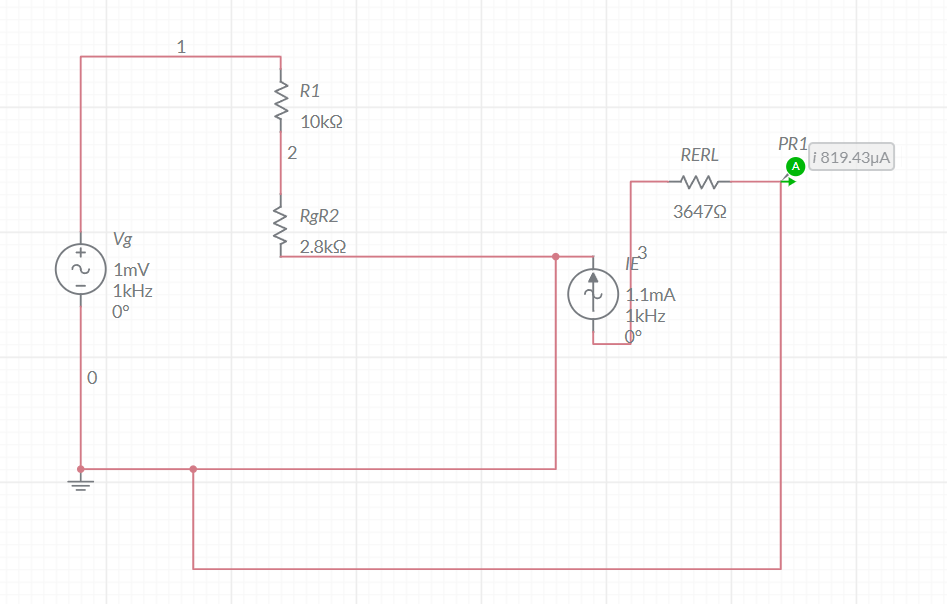
\includegraphics[width=1\textwidth]{Simulacao21.png}
    \large \textbf{Figura 9 - Simulação da Questão 2}
\end{figure}

\begin{figure}[H]
    \centering
    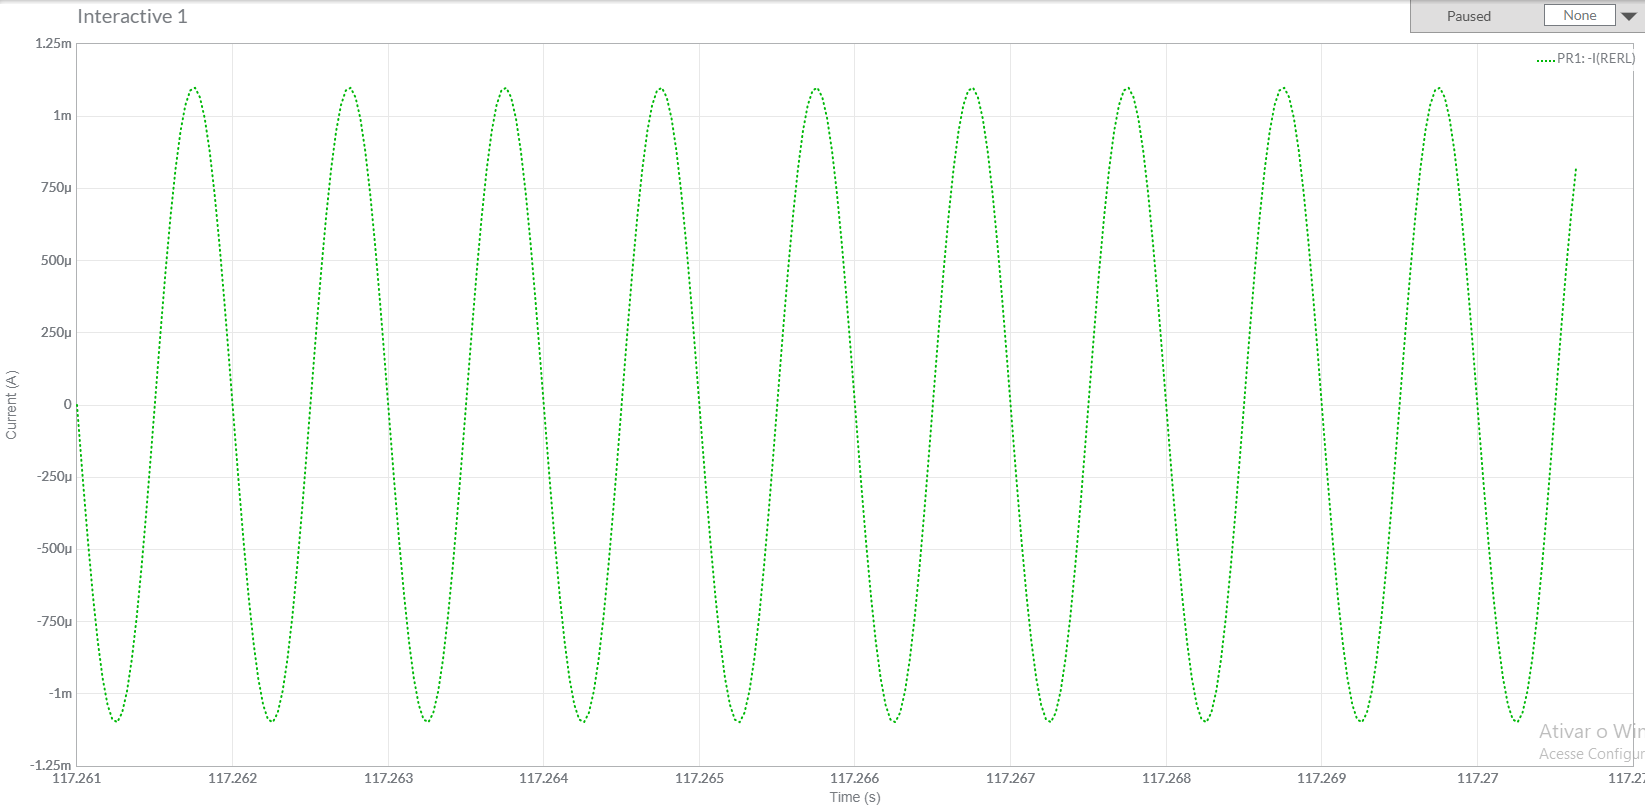
\includegraphics[width=1\textwidth]{Simulacao22.png}
    \large \textbf{Figura 10 - Simulação da Questão 2}
\end{figure}

\chapter{Questão 3}
\section{}

\subsection{Simplificação da Polarização por Divisor de Tensão}
\begin{center}
    \begin{tikzpicture}
    	% Paths, nodes and wires:
    	\draw node[ground] at (3, 5.625) {};
    	\draw node[ground] at (4.5, 5.625) {};
    	\draw node[ground] at (6, 5.625) {};
    	\draw (3, 5.625) to[american resistor, l={$R2$}, label distance=0.02cm] (3, 7.875);
    	\draw (4.5, 5.5) to[american resistor, l={$RE$}, label distance=0.02cm] (4.5, 7);
    	\draw node[npn] at (4.5, 9) {};
    	\draw (3, 7.875) -| (3, 9) -- (3.66, 9);
    	\draw (3, 9.77) to[american resistor, l={$R1$}, label distance=0.02cm] (3, 11.52);
    	\draw (4.5, 9.77) to[american resistor, l={$RC$}, label distance=0.02cm] (4.5, 11.52);
    	\draw (3, 11.52) -- (4.5, 11.52);
    	\draw (3, 9.77) -| (3, 9);
    	\draw (6, 9.375) to[battery, l={$VCC$}, label distance=0.02cm] (6, 8.625);
    	\draw (6, 5.625) -| (6, 8.625);
    	\draw (4.5, 11.52) -| (6, 11.5) -| (6, 9.375);
    	\draw node[circ] (N1) at (3, 9) {} node[anchor=south east] at (N1.north west){$VBB$};
    	\draw (4.5, 8.23) to[american resistor, l_={$re$}, label distance=0.02cm] (4.5, 7);
    \end{tikzpicture}
    \\
    \textbf{Figura 11 - Circuito Elétrico Simplificado}
\end{center}

\subsection{Dados do Circuito}
\begin{itemize}
    \item $V_{CC} = 10\,V$ 
    \item $R_{1} = 10\,{k}\Omega$ 
    \item $R_{2} = 2,2\,{k}\Omega$
    \item $R_{C} = 3,6\,{k}\Omega$
    \item $R_{E} = 820 \ \Omega$
    \item $R_{L} = 10\,{k}\Omega$
    \item $R_{G} = 600 \ \Omega$
    \item $r_{e} = 180 \ \Omega$
    \item $\beta = 100$
\end{itemize}
    
\subsection{Cálculo de $V_{BB}$}
\[
V_{BB} = \frac{R_{2}}{R_{1} + R_{2}} \cdot V_{CC}
\implies
V_{BB} = \frac{2,2k}{10k + 2,2k} \cdot 10
\implies
\tikz[baseline]{\node[draw=red, thick, rounded corners] {$V_{BB} = 1,8\,\text{V}$};}
\]

\subsection{Cálculo de $I$}
\[
I = \frac{V_{CC}}{R_{1} + R_{2}} \implies
I = \frac{10}{10k + 2,2k} \implies
\tikz[baseline]{\node[draw=red, thick, rounded corners] {$I \approx 0,82\,\text{mA}$};}
\]

\subsection{Cálculo de $V_{B}$}
\[
V_{B} = R_{2} \cdot I \implies V_{B} = 2,2k \cdot 0,82 \therefore \tikz[baseline]{\node[draw=red, thick, rounded corners] {$V_{B} \approx 1,8\,\text{V}$};}
\]

% \subsection{Cálculo de $I_{E}$}
% Adotando $V_{BE} = 0,7\,V$ e aplicando LKT na malha sentido $R_{2}$$V_{BB}$$R_{E}$, tem-se:
% \[
% V_{BB} - V_{BE} - R_{E}I_{E} = 0 
% \implies 
% I_{E} = \frac{V_{BB} - V_{BE}}{R_{E}} 
% \implies 
% I_{E} = \frac{1{,}8 - 0{,}7}{1\,\text{k}} 
% \therefore 
% \tikz[baseline]{\node[draw=red, thick, rounded corners] {$I_{E} = 1{,}1\,\text{mA}$};}
% \]

\subsection{Cálculo de $V_{E}$}
Sabe-se que:
\[
V_{E} = V_{BB} - V_{BE} \implies V_{E} = 1,8 - 0,7 \therefore \tikz[baseline]{\node[draw=red, thick, rounded corners] {$V_{E} = 1{,}1\,\text{V}$};}
\]

\subsection{Cálculo de $I_{E}$}
\[
I_E = \frac{V_E}{R_E + r_e} \implies I_E = \frac{1{,}1}{820 + 180}  \therefore \tikz[baseline]{\node[draw=red, thick, rounded corners] {$I_E = 1{,}1\,\text{mA}$};}
\]

\subsection{Cálculo de $I_{C}$}
Devido ao fato de que $\beta \geq 100$ $\therefore I_C \approx I_E$
\[
\tikz[baseline]{\node[draw=red, thick, rounded corners] {$I_{C} = 1{,}1\,\text{mA}$};}
\]

\subsection{Cálculo de $I_{B}$}
\[
I_{B} = \frac {I_{C}} \beta \implies I_{B} = \frac {1,1m} {100} \therefore \tikz[baseline]{\node[draw=red, thick, rounded corners] {$I_{B} = 0{,}011\,\text{mA}$};}
\]

\subsection{Cálculo de $V_{C}$}
Sabe-se que:
\[
V_{C} = V_{CC} - R_{C} I_{C} \implies V_{C} = 10 - 3,6k \cdot 1,1m \therefore \tikz[baseline]{\node[draw=red, thick, rounded corners] {$V_{C} = 6{,}04\,\text{V}$};}
\]

\subsection{Cálculo de $V_{CE}$}
Sabe-se que:
\[
V_{CE} = V_{C} - V_{E} \implies V_{CE} = 6,04 - 1,1 \therefore \tikz[baseline]{\node[draw=red, thick, rounded corners] {$V_{CE} = 4{,}94\,\text{V}$};}
\]

\subsection{Comprovação através do gráfico do funcionamento como amplificador}
\[
I_{C_{\text{máx}}} = \frac {V_{CC}}{R_{C} + R_{E}} \implies I_{C_{\text{máx}}} = \frac {10}{3,6k + 820} \therefore \tikz[baseline]{\node[draw=red, thick, rounded corners] {$I_{C_{\text{máx}}} \approx 2{,}26\,\text{mA}$};}
\]
\[
V_{CE_{\text{corte}}} \approx V_{CC} \therefore V_{CE_{\text{corte}}} \approx 10\,V
\]

\begin{center}
    \begin{tikzpicture}
        % Eixos
        \draw[->] (0,0) -- (5.5,0) node[right] {$V_{CE}\,\text{(V)}$};
        \draw[->] (0,0) -- (0,5) node[above] {$I_C\,\text{(mA)}$};

        % Linha do transistor
        \draw[thick] (4,0) -- (0,4) node[left] {$I_{C_{\text{máx}}}$};

        % Ponto de corte
        \node at (4,-0.3) {$V_{CE_{\text{corte}}}$};

        % Linhas tracejadas do ponto de operação
        \draw[dashed] (0,1.8) -- (2.14,1.8);  % linha horizontal
        \draw[dashed] (2.14,0) -- (2.14,1.8); % linha vertical

        % Rótulos dos valores
        \node[left] at (0,1.8) {$1{,}1$};
        \node[below] at (2.14,0) {$4{,}94$};

        % Ponto de operação
        \node at (2.14,1.8) {•}; % ponto marcado
    \end{tikzpicture}

    \\  % pula uma linha (ajustável: 1em, 2ex, etc.)

    \large \textbf{Figura 12 - Gráfico $I_C$ x $V_{CE}$}
\end{center} Devido ao fato do ponto estar em cima da linha de carga e não estar nas extremidades ($I_{C_{\text{máx}}}$ e $V_{CE_{\text{corte}}}$), o transistor se comporta como um amplificador.

\section{}
Adotando $\pi = 3,14$ e não atribuindo valor à frequência (forma literal)

\subsection{Cálculo do $R_{1} || R_{2}$}
\[
R_{1} || R_{2} = \frac{R_{1} \cdot R_{2}}{R_{1} + R_{2}} \implies R_{1} || R_{2} = \frac{10k \cdot 2,2k}{10k + 2,2k} \therefore \tikz[baseline]{\node[draw=red, thick, rounded corners] {$R_{1} || R_{2} \approx 1803{,}28\,\Omega$};}
\]

\subsection{Cálculo do $R_{eqC1}$}
\[
R_{eqC1} = R_{G} + (R_{1} || R_{2}) \implies R_{eqC1} = 600 + 1803{,}28 \therefore \tikz[baseline]{\node[draw=red, thick, rounded corners] {$R_{eqC1} \approx 2403{,}28\,\Omega$};}
\]

\subsection{Cálculo do $C_{1}$}
\[
C_{1} \geq \frac{1}{2\pi0,1R_{eqC1}f} \implies C_{1} \geq \frac{1}{2\pi0,1(2403,28)f} \therefore \tikz[baseline]{\node[draw=red, thick, rounded corners] {$C_{1} \geq (6{,}63f)\,\text{mF}$};}
\]

\subsection{Cálculo do $C_{2}$}
\[
C_{2} \geq \frac{1}{2\pi0,1R_{E}f} \implies C_{2} \geq \frac{1}{2\pi0,1(820)f} \therefore \tikz[baseline]{\node[draw=red, thick, rounded corners] {$C_{2} \geq (1{,}94f)\,\text{mF}$};}
\]

\subsection{Cálculo do $R_{C} || R_{L}$}
\[
R_{C} || R_{L} = \frac{R_{C} \cdot R_{L}}{R_{C} + R_{L}} \implies R_{C} || R_{L} = \frac{3,6k \cdot 10k}{3,6k + 10k} \therefore \tikz[baseline]{\node[draw=red, thick, rounded corners] {$R_{C} || R_{L} \approx 2647{,}06\,\Omega$};}
\]

\subsection{Cálculo do $C_{3}$}
\[
C_{3} \geq \frac{1}{2\pi0,1(R_{C} || R_{L})f} \implies C_{3} \geq \frac{1}{2\pi0,1(2647,06)f} \therefore \tikz[baseline]{\node[draw=red, thick, rounded corners] {$C_{3} \geq (6{,}02f)\cdot 10^{-4}\,\text{F}$};}
\]

\section{}

\subsection{Cálculo de $re'$}
\[
re' = \frac{25mV}{I_{E}} \implies re' = \frac{25mV}{1,1mA} \therefore \tikz[baseline]{\node[draw=red, thick, rounded corners] {$re' \approx 22{,}72\,\Omega$};}
\]

\subsection{Cálculo da impedância de entrada da base ($Z_{in_{\text{B}}}$)}
\[
Z_{in_{\text{B}}} = \beta \cdot re' \implies Z_{in_{\text{B}}} = 100 \cdot 22,72 \therefore \tikz[baseline]{\node[draw=red, thick, rounded corners] {$Z_{in_{\text{B}}} = 2{,}272\,k\Omega$};}
\]

\subsection{Cálculo do $R_{B}$}
\[
R_{B} = R_{1} || R_{2} \implies R_{B} = \frac{R_{1} \cdot R_{2}}{R_{1} + R_{2}} \implies R_{B} = \frac{10k \cdot 2,2k}{10k + 2,2k} \therefore \tikz[baseline]{\node[draw=red, thick, rounded corners] {$R_{B} \approx 1803{,}28\,\Omega$};}
\]

\subsection{Cálculo da impedância de entrada ($Z_{in}$)}
\[
Z_{in} = R_{G} + (R_{B} || Z_{in_{\text{B}}}) \implies Z_{in} = 600 + \frac{1,80328k \cdot 2,272k}{1,80328k + 2,272k} \therefore \tikz[baseline]{\node[draw=red, thick, rounded corners] {$Z_{in} \approx 1{,}6\,k\Omega$};}
\]

\subsection{Cálculo da impedância de saída}
\[
Z_{out} \approx R_{C} \therefore \tikz[baseline]{\node[draw=red, thick, rounded corners] {$Z_{out} = 3{,}6\,k\Omega$};}
\]Sim, temos um amplificador de pequenos sinais devido, não só a análise das impedâncias de entrada e saída, mas também pelo fato de $V_{g} = 1\,mV$, valor esse tido como pequeno.

\section{}

\subsection{Cálculo de $r_{c}$}
\[
r_{c} = R_{c} || R_{L} \implies r_{c} = \frac{3,6k \cdot 10k}{3,6k + 10k} \therefore \tikz[baseline]{\node[draw=red, thick, rounded corners] {$r_{c} \approx 2647{,}06\,\Omega$};}
\]

\subsection{Cálculo de $re'$}
\[
r_e' = r_e + R_E \implies r_e' = 180 + 820 \therefore\tikz[baseline]{\node[draw=red, thick, rounded corners] {$r_e' = 1000 \ \Omega$};}
\]

\subsection{Cálculo do ganho de sinal}
\[
A_{v} = \frac{r_{c}}{re'} \implies A_{v} = \frac{2647,06}{1000} \therefore \tikz[baseline]{\node[draw=red, thick, rounded corners] {$A_{v} \approx 2{,}64706$};}
\]

\section{}
\subsection{Esboço}
\begin{center}
\begin{tikzpicture}[scale=1.2]
    % Eixos
    \draw[->] (-1.5,0) -- (5.5,0) node[right] {$t\,\text{(s)}$};
    \draw[->] (0,-1.5) -- (0,1.8) node[above] {$V(V)$};

    % Parte tracejada à esquerda
    \draw[dashed, domain=-1.5:0, samples=100, smooth] 
        plot(\x, {sin(2*pi*\x r)});

    % Parte principal (contínua)
    \draw[thick, domain=0:4.5, samples=200, smooth] 
        plot(\x, {sin(2*pi*\x r)});

    % Parte tracejada à direita
    \draw[dashed, domain=4.5:5.2, samples=100, smooth] 
        plot(\x, {sin(2*pi*\x r)});
\end{tikzpicture}
\\
\large \textbf{Figura 13 - Gráfico $V$ x $t$}
\end{center}

\subsection{Simulação no MULTISIM}
\begin{figure}[H]
    \centering
    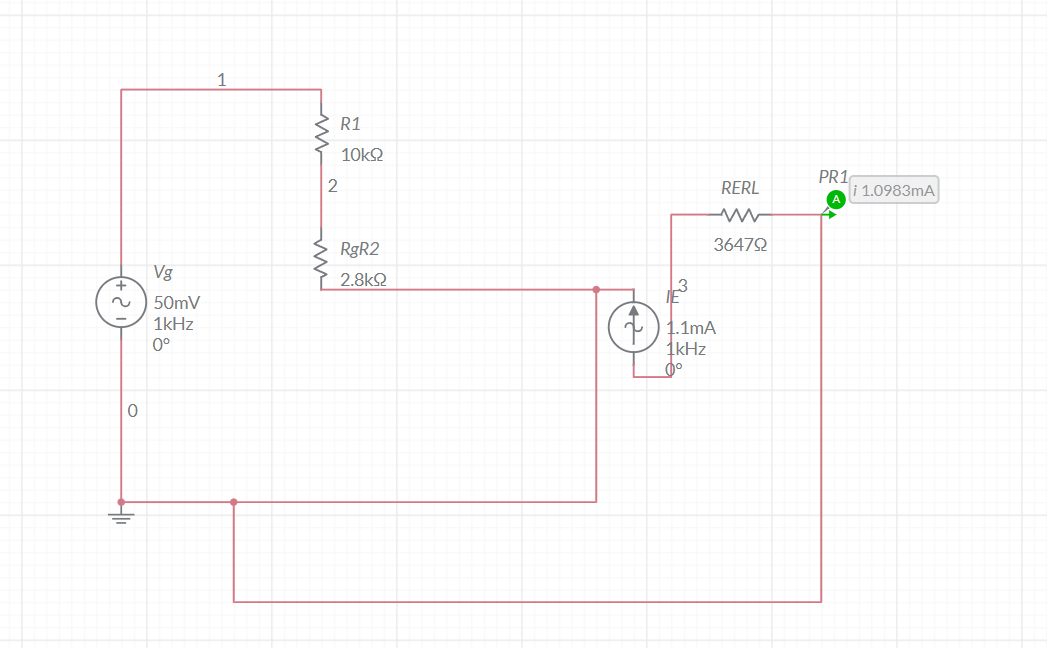
\includegraphics[width=1\textwidth]{Simulacao31.png}
    \large \textbf{Figura 14 - Simulação da Questão 3}
\end{figure}

\begin{figure}[H]
    \centering
    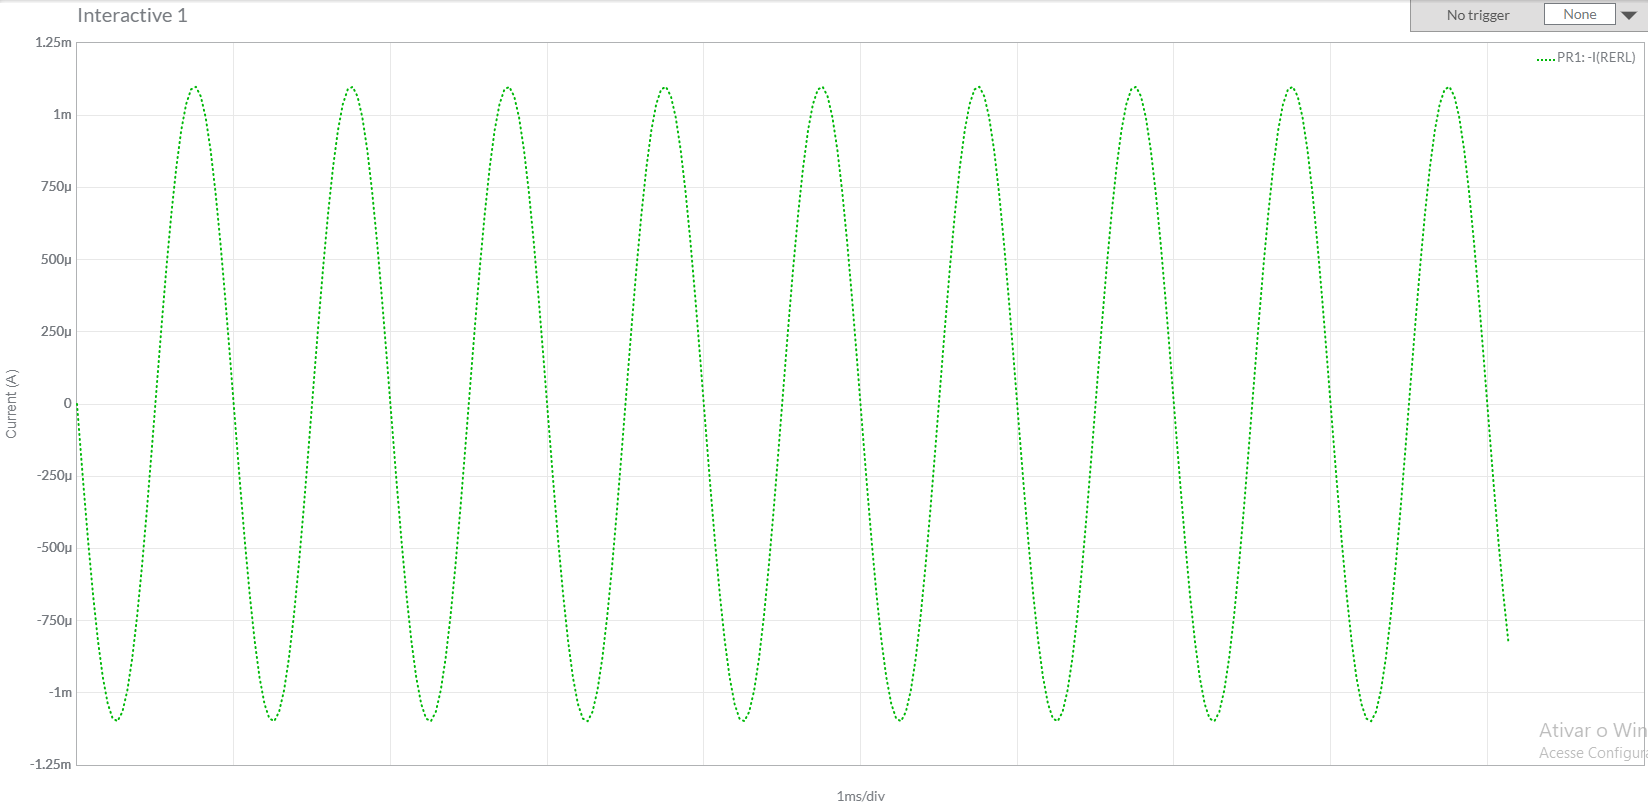
\includegraphics[width=1\textwidth]{Simulacao32.png}
    \large \textbf{Figura 15 - Simulação da Questão 3}
\end{figure}

\end{document}
